%\pagenumbering{arabic}
\section{开发技术选择}

\subsection{物联网通讯协议  MQTT}

在本系统前期的网络数据传输技术选型对比了TCP/UDP/JSON/MQTT等传输协议或方式的优缺点,综合考虑选择了MQTT(Message Queuing Telemetry Transport,消息队列遥测传输协议)作为本次客户端节点和服务端节点数据交互的协议。其协议广泛地应用在机器对计算机( m2m )/物联网( iot )的多层次应用互联网连接协议,使用了极其轻质级的分布式发布/订阅二进制消息模型的通信。对于那些需要较小的代码所占用的空间和或者在网络上带宽很大时候非常宝贵的数据连接非常有用,是专门针对受限的设备(电池功率很大的移动应用)和低频带宽、高时间延迟或不可靠环境中进行无线通信而开发和设计的。不仅为新兴的"机器到机器"( m2m )或物联网( iot )全球范围内的世界各地人群提供了连接,还被广泛应用于通过卫星链路和传感器与代理人进行通信、与医疗服务提供商的电话拨号互联网连接以及家庭自动化和微型设备等场景。
\\ 相对与其他协议,MQTT具有以下特性:
\\1. 底层基于 tcp / ip (或者 udp )协议进行传输,采用了发布/订阅模式的二进制消息模式,提供一对多的信息发布。
\\2. 控制数据传输包的报头结构简单,第一个字节报头为固定的控制报头,第二个字节为自动心跳式控制报文,最小化了数据传输的成本开销与无线协议之间的数据交换,有效地大大降低了无线网络的传输流量。
\\3. 消息QoS支持,可靠性传输保证(TCP协议传输)
\\4. 使用Last Will和Testament特性通知有关各方客户端异常中断的机制。

MQTT 协议主要有三大核心角色:发布者(Publisher)、Broker代理服务器(转发者)、订阅者(Subscriber)。其中消息的发布者和订阅者都是客户端角色,消息代理是服务器,消息发布者可以同时是订阅者。

MQTT客户端身兼二职:既可以是发布者角色,又可以是订阅者角色。一个使用MQTT协议的应用程序或者设备就是一个MQTT 客户端,工作时它需要主动去连接到代理服务器\upcite{丁宜2016基于移动医疗的脉搏信号监测系统的设计与实现}。

MQTT网络服务器也被广泛简称它作为"消息代理"网络服务器(broker),可以也被认为为它是一个独立的网络应用程序或一台移动设备,它通常来说是分别放在面向消息发送信息的新闻发布者和消息订阅供应商之间,具有以下几个功能:
即时接收和处理建立不同来自两个客户端的即时网络消息链路并与其客户建立即时通讯网络链路,
接收到来自消息新闻发布者的消息主题(topic)并将其主题转发给消息订阅供应商,处理一些出现在不同来自两个客户端的网络消息例如订阅和
退订请求。
向订阅的客户转发相应地主题(Topic)。
其具体交互流程如下图\ref{fig:3-1}所示:

\begin{figure}[htbp]
	\centering
	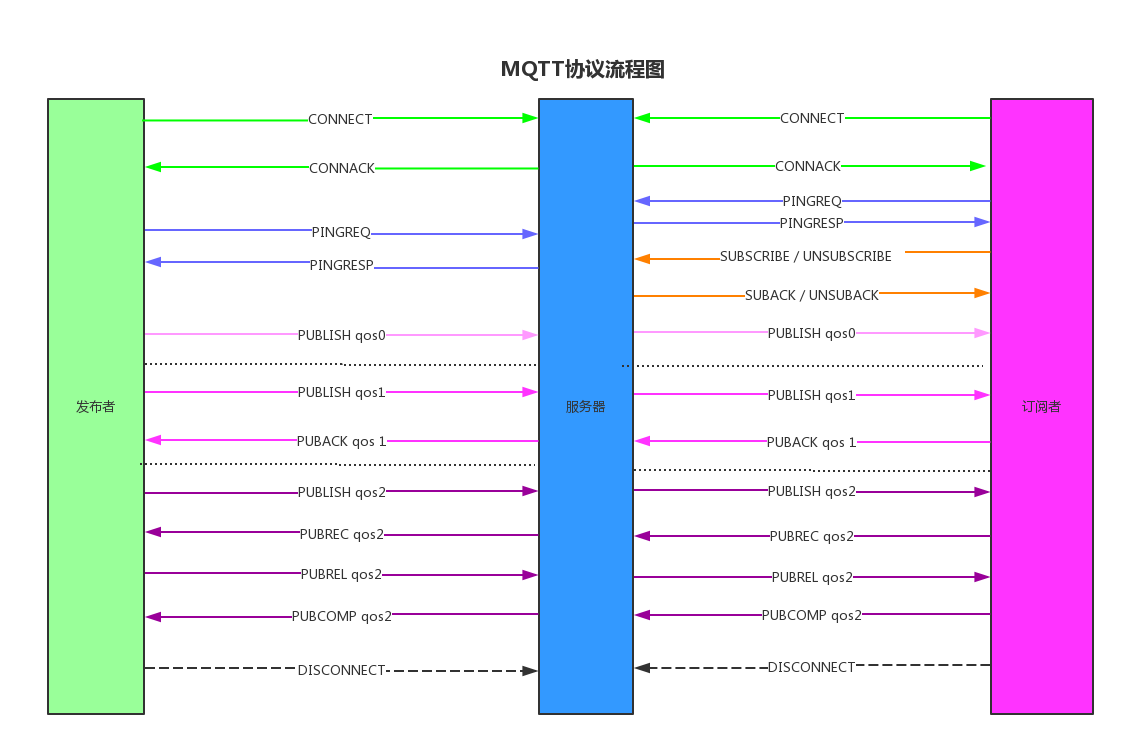
\includegraphics[width=1\linewidth]{figure/3-1}
	\caption{MQTT协议流程图}
	\label{fig:3-1}
\end{figure}


\subsection{关系性数据库 MySQL}


数据库(Database)是按照数据结构来组织、存储和管理数据的仓库。
我们也可以将数据存储在文件中,但是在文件中读写数据速度相对较慢。
所以,现在我们使用关系型数据库管理系统(RDBMS)来存储和管理大数据量。所谓关系式模型数据库,就是指建立在传统的关系式模型基础上的一种数据库,借助集合代数等传统的数学概念和技术手段来收集和处理整个数据库系统中的各种数据。
\\RDBMS 即关系数据库管理系统(Relational Database Management System)的特点:

1.数据以表格的形式出现

2.每行为各种记录名称

3.每列为记录名称所对应的数据域

4.许多的行和列组成一张表单

5.若干的表单组成database


MySQL 是一个关系型数据库管理系统,由瑞典 MySQL AB 公司开发,目前属于 Oracle 公司。MySQL 是一种关联数据库管理系统,关联数据库将数据保存在不同的表中,而不是将所有数据放在一个大仓库内,这样就增加了速度并提高了灵活性。
MySQL具有以下特性:
\begin{itemize}
	\item  MySQL 本身是自由软件开源,目前已经附属于 oracle 旗下的产品。
	\item MySQL 支持大型的数据库。可以处理拥有上千万条记录的大型数据库。
	\item MySQL 使用标准的 SQL 数据语言形式。
	\item MySQL 可以运行于多个系统上,并且支持多种语言。这些编程语言囊括了几乎常见的编程语言。
	\item MySQL 支持大型数据库,支持 5000 万条记录的数据仓库,32 位系统表文件最大可支持 4GB,64 位系统支持最大的表文件为8TB。
	\item MySQL 是可以定制的,采用了 GPL 协议,可针对源码进行定制化开发。
\end{itemize}

\subsection{Python开发语言 Flask模块}

Flask 一直被人称为它就是 python 中一种轻量级且具有自己定制功能的可以进行定制的框架,其优点是核心简单,相比其他的框架更加灵活轻便,也更容易掌握。

Flask框架核心简单,同时在使用过程同样可以保持功能的丰富与扩展性,用户在使用Flask开发网站时,可以根据自己的需求添加不同的功能,各种强大的插件库可以让用户完全按照自己的意愿开发出功能强大的WEB网站。

\begin{lstlisting}[title=代码 3-1:Flask简单示例]
from flask import Flask
app = Flask(__name__)
@app.route('/')
def index():
    return 'Hello World'
\end{lstlisting}

仅仅5行代码,就可以在浏览器中显示一个Hello World响应。所以Flask的其中一个优势再明显不过了:简洁。且不说Java的Web框架Spring,就说同样使用Python的框架Django,写一个Hello World程序也得10行代码。

第一行,导入包。

第二行,创建对象。

第三行,创建路由。

第四行、第五行,视图函数。

\subsection{SQLAlchemy---对象关系映射器(ORM)}

SQLAlchemy是一个功能非常强大的库,用于在Python中处理关系数据库。代替手工编写SQL查询,我们可以使用普通的Python对象来表示数据库表并执行查询。这种方法有很多好处,如下代码所示:

\begin{lstlisting}[title=DHT11数据表对象数据表模型]
class Dht11(PaginatedAPIMxin, db.Model):
__tablename__ = 'Dht11'
id = db.Column(db.Integer, primary_key=True)  #卡片存储收到MQTT数据的序号
temperature = db.Column(db.String(48), index=True) #存储MQTT数据中温度
humidity = db.Column(db.String(48), index=True)  #存储MQTT数据中湿度
timestamp = db.Column(db.DateTime, index=True, default=datetime.utcnow) #存储当前收到数据的时间戳
card_id = db.Column(db.Integer, db.ForeignKey('boards.id')) #对应的卡片ID

def __repr__(self):   #__repr__方法,它用于生成Dht11类实例的辅助显示内容
	return '<temp:{0}, humidity:{1}'.format(self.temperature, self.humidity)

def to_dict(self):  #单个对象方法
	data = {
		'id_from_db': self.id,
		'owner_email': str(User.query.get_or_404(self.card_id).email),
		'from_card_id': self.card_id,
		'value_created_at': self.timestamp,
		'temperature': self.temperature,
		'humidity': self.humidity,
		'_links': {
			(self.card_id).id) # user_id
			}
		}
	return data
\end{lstlisting}

通过ORM方法的使用很容易的构建了返回对象的数据格式

与手工编写SQL查询相反,我们可以使用普通的Python对象来表示数据库表,并执行查询。如下,该方法有很多的优点:

应用程序可以完全用Python开发。

数据库引擎之间的细微差别被抽象掉了。这使可以像处理轻量级数据库一样进行操作,例如,使用SQLite进行本地开发和测试,然后切换到专为生产中的高负载而设计的数据库(例如PostgreSQL)。

数据库错误不太常见,因为您的应用程序和数据库服务器之间现在存在两层:Python解释器本身(这将捕获明显的语法错误)和SQLAlchemy,后者具有定义良好的API和自己的错误检查层。

由于SQLAlchemy的工作单元模型有助于减少不必要的数据库往返次数,因此数据库代码可能会变得更加高效。SQLAlchemy还具有有效地预取相关对象的功能,称为预先加载。

对象关系映射(Object Relational Mapping,ORM)使代码更具可维护性,这被称为“不要重复自己”(DRY)。假设将列添加到模型中。使用SQLAlchemy,只要您使用该模型,它将可用。另一方面,如果整个应用程序中都散布着手写的SQL查询,则需要一次更新一次每个查询,以确保包含新列。SQLAlchemy可以帮助避免SQL注入漏洞。

出色的库支持:有很多有用的库可以直接与SQLAlchemy模型一起使用,以提供诸如维护接口和RESTful API之类的东西。

应用可以完全使用Python开发。


\subsection{RESTful 架构开发方式}
REST全称是Representational State Transfer,中文意思是表述(通常译为表现层状态转移)。 REST本身并没有创造新的技术、组件或服务,而隐藏在RESTful背后的理念就是使用Web的现有特征和能力, 更好地使用现有Web标准中的一些准则和约束。虽然REST本身受Web技术的影响很深, 但是理论上REST架构风格并不是绑定在HTTP上,只不过目前HTTP是唯一与REST相关的实例。 所以我这里描述的REST也是通过HTTP实现的REST。

REST全称是表述性状态转移,那究竟指的是什么的表述? 其实指的就是资源。任何事物,只要有被引用到的必要,它就是一个资源。资源可以是实体(例如手机号码),也可以只是一个抽象概念(例如价值) 。下面是一些资源的例子:
\begin{itemize}
	\item 某用户的手机号码
	\item 某用户的个人信息
\end{itemize}

要让一个资源可以被识别,需要有个唯一标识,在Web中这个唯一标识就是URI(Uniform Resource Identifier)。

URI既可以看成是资源的地址,也可以看成是资源的名称。URI的设计应该遵循可寻址性原则,具有自描述性,需要在形式上给人以直觉上的关联。这里以github网站为例,给出一些还算不错的URI:
\begin{itemize}
	\item https://github.com/git/git
	\item https://github.com/git/git/blob/master/block-sha1/sha1.h
	\item https://github.com/git/git/commit/a5dg45d5y1n88
	\item https://github.com/git/git/pulls
	\item https://github.com/git/git/pulls?state=closed
\end{itemize}

1. REST描述的是在网络中client和server的一种交互形式;REST本身不实用,实用的是如何设计 RESTful API(REST风格的网络接口);
2. Server提供的RESTful API中,URL中只使用名词来指定资源,原则上不使用动词。“资源”是REST架构或者说整个网络处理的核心。
以本次系统开发的接口举例如下:
\begin{itemize}
	\item http://arduino.deconf.xyz/api/users/1/cards/: 获取用户的全部卡片信息; 
	\item http://arduino.deconf.xyz/api/cards/1/: 获取卡片编号为1的所有信息;
	\item http://arduino.deconf.xyz/api/cards/1/dht11/: 获取卡片1的dht11传感器的全部信息;
\end{itemize}

3. 使用了 HTTP 协议里的一个可变动词组来进行替换实现对一个资源的直接添加,修改,删除。即通过表示 HTTP 一个状态动词可以用来直接实现对所有资源的状态的更改:
get 用来自动获得所有资源,
post 用来自动创建新的所有资源(也就是说它有时可以被广泛地认为用来自动更新包含的所有资源)
, put 可以用来修改和更新资源,
delete 可以用来修改和删除。
其过程如图 \ref{fig3-2} 所示:
\begin{figure}[H]
	\centering
	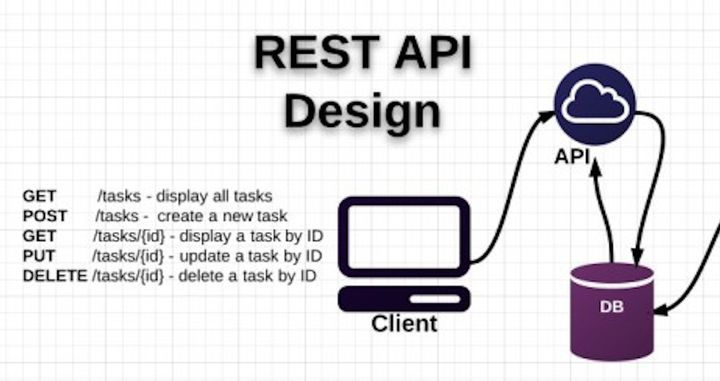
\includegraphics[width=0.85\linewidth]{figure/3-2}
	\caption{RESTful 设计理念图}
	\label{fig:3-2}
\end{figure}

通过日常使用的RESTful,系统就这样可以轻松实现:前后两个端的网络分离,减少了网络流量。安全的特性问题大部分都可以集中应用到文件接口上。因为接口只接受json的各种json文件格式,防止了一些用户随意注入文件类型等的安全特性问题。前端不用需要进行数据有关化,后端仅仅需要负责一个前端数据的综合处理,而且前端的各种表现形式也完全可以直接选择为任何一种新的前端表现语言(android,ios,html5)。前端与后端的交互操作开发人员更为容易专注于各自的交互开发,仅仅用户只需一个基于接口的开发文档文件即可轻松地直接完成前后端的交互,而且不用过分担心过多的相互信息泄漏。
服务器的网站性能得到优化:由于其网站前端静态的一个网页,通过HTTP 即时方式获取,服务器的主要处理压力就已经落到了前端接口上。
